\def\Thisfile{Chapter4.tex}
\def\Thisfiledate{2020/02/24}
\typeout{***** `\Thisfile' <\Thisfiledate> *****}
\NeedsTeXFormat{LaTeX2e}
\documentclass[12pt]{article}
\usepackage{ifthen,pifont,latexsym}
\usepackage[T1]{fontenc}
\usepackage{times,avant}
%%\usepackage{mathrsfs}
%\usepackage[mtpluscal,mtplusscr,T1]{mathtime}
\usepackage[round,authoryear]{natbib}
%%
\usepackage[pdftex]{graphicx}
%%
\def\Includefigs{true}
%%\usepackage{amsmath}
%%
%% \usepackage{draftmark}\markdraftpage
%%
%%%%%%%%%% Other preamble commands here ...
%%
\textwidth 6.5in
\oddsidemargin 0in
\topmargin -.25in
\textheight 8.5in
%%
\def\rfeqn#1{(\ref{eq.#1})}
\def\vs#1{\vspace{#1\baselineskip}}
\def\HeadSpace{\vs{.17}}
\def\BoldHead#1{\HeadSpace\textbf{#1}}
\def\ItalHead#1{\HeadSpace\textit{#1}}
\def\UlHead#1{\HeadSpace\underline{#1}}
\def\floatpagefraction{.7}
%%
\newenvironment{descz}{\begin{description}\def\itemsep{0in}}%%
{\end{description}}
\newenvironment{itemz}{\begin{itemize}\def\itemsep{0in}}%%
{\end{itemize}}
\newenvironment{enumz}{\begin{enumerate}\def\itemsep{0in}}%%
{\end{enumerate}}
\newcommand{\m}{\ensuremath{\mathbf{\mu}}}
\newcommand{\s}{\ensuremath{\mathbf{\Sigma}}}

%%\input acronyms.tex
%%
%% Def's and macros
%%
% \mathscr changed to \mathcal in the following by APS
\def\DB{\ensuremath{\mathbf{D}}} %% Database
\def\QS{\ensuremath{\mathscr{Q}}} %% Query space
\def\DR{\ensuremath{\mathbf{DR}}} %% Disclosure risk
\def\DU{\ensuremath{\mathbf{DU}}} %% Data utility
\def\DD{\ensuremath{\mathbf{DD}}} %% Data distortion
\def\RS{\ensuremath{\mathbf{R}}} %% Release space
\def\DBORIG{\ensuremath{{D}_{\mathrm{orig}}}} %% Database
\def\DBPOST{\ensuremath{\mathscr{D}_{\mathrm{post}}}} %% Database
\def\DBREL{\ensuremath{D_{\mathrm{rel}}}} %% Released database
%% Methods
\def\NOI{{\tt Noise}}
\def\MICZ{{\tt Micz}}
\def\MICP{{\tt Micp}}
\def\MICM{{\tt Micm_all}}
\def\MICI{{\tt Micir}}
\def\MIC7{{\tt Micm_groups}}
\def\RESAMP{{\tt Resamp}}
\def\RANK{{\tt Rank}}
%% Utility measures
\def\LR{\ensuremath{\mathbf{LR}}} %% Likelihood ratio
\def\KL{\ensuremath{\mathbf{KL}}} %% KL measure
\def\IO{\ensuremath{\mathbf{IO}}} %% interval overlap measure
\def\EO{\ensuremath{\mathbf{EO}}} %% ellipsoid overlap measure
%\def\argmax{\operatornamewithlimits{arg\max}}
\def\SDL{statistical disclosure limitation (SDL)%%
    \gdef\SDL{SDL}}

\begin{document}

\title{Chapter 4
\\
Data Utility}

%\author{ A. Oganian\thanks{National Center for Health Statistics, CDC, Hyattsville, MD, USA}
%}

\maketitle

\begin{abstract}
When releasing data to the public, statistical agencies and survey
organizations typically alter data values in order to protect the
confidentiality of survey respondents' identities and attribute
values.  To select among the wide variety of data alteration
methods, agencies require tools for evaluating the utility of
proposed data releases.  Such utility measures can be combined
with disclosure risk measures to gauge risk-utility tradeoffs of
competing methods.  Some examples of utility metrics are presented in this Chapter.
A  decision-theoretic formulation for evaluating
disclosure limitation procedures based on utility and risk metrics is outlined
as well. Finally, examples of utility assessments of certain families of SDL methods are 
given. 


\end{abstract}

\section{Introduction}\label{sec.intro}

As it was described in Chapter 3, there is a wide range of \SDL\ techniques.
These \SDL\ methods can be implemented with differing degrees of
intensity.  Generally, increasing the amount of alteration
decreases the risk of disclosure, but it also decreases the
accuracy of inferences obtainable from the released data, often
referred to as data utility \citep{Hund10}.

So,  \SDL\ practitioner needs to decide which technique, and with what
degree of intensity to use in a particular setting of data release. 
In general the approach to this problem is to employ risk-utility formulations. We assume
below that each candidate release $R$ can be characterized by a quantified
\textit{disclosure risk} $\DR (R)$ and \textit{data utility} $\DU
(R)$.  Examples of $\DU(R)$ metrics are given in Section \ref{du_metrics}.
The particular released data, $DB_{REL}$, can be selected from
the candidates in one of two ways. The first is to maximize
utility subject to an upper bound on risk, by solving an
optimization problem of the form
\begin{equation}\label{eq.opt}
\begin{array}{l}
DB_{REL} = {\arg\max}_{R \in \RS} \DU (R) \\[1ex]
\mbox{s.t. } \DR(R) \leq \alpha
\end{array}
\end{equation}
where \RS\ is the set of all possible releases. 

The second and more flexible approach is to define \textit{risk-utility
frontiers} using the partial order $\preceq_{\mathrm{RU}}$ defined
by
\begin{equation}\label{eq.rupo}
R_1 \preceq_{\mathrm{RU}} R_2 \Leftrightarrow \DR(R_2) \leq
\DR(R_1) \qquad\mbox{and}\qquad \DU(R_2) \geq \DU(R_1).
\end{equation}

When $R_1 \preceq_{\mathrm{RU}} R_2$, the $R_2$ is preferred to
$R_1$ because it has both lower disclosure risk and higher
utility. Only candidate releases on the risk-utility frontier of
maximal elements of \RS\ with respect to the partial order
(\ref{eq.rupo}) need be considered further: for any other
candidate, some element of the frontier has lower risk
\textit{and} higher utility. Calculation of the frontier can be
done using existing algorithms for finding the maxima in a set of
vectors \citep{kung-luccio-preparata75}. 


The choice among the SDL methods lying on the risk-utility
frontier lies with the data disseminator. To illustrate the first approach
described above, consider Figure \ref{fig.ruplot}, where each point
represents some SDL method characterized in terms of Utility and Risk 
measured according to certain metrics on the horizontal and vertical axes respectively.
If the risk threshold were $10\%$ (in some settings, not a very conservative value), 
then a method denoted as \NOI\ would be the preferred SDL. It is also clear from Figure \ref{fig.ruplot} that compared to \MICZ\ or \NOI\, \MICI\ produces only a minor increase
in utility at an enormous cost in terms of disclosure risk. Similarly,
\RANK\ yields only a modest improvement in disclosure
risk over \MICP\ and \NOI\, but incurs an immense
penalty in terms of data utility. Thus, in a scenario represented by Figure \ref{fig.ruplot}
 the disseminator  might prefer \NOI\ or \MICP\ .

\begin{figure}
\begin{center}
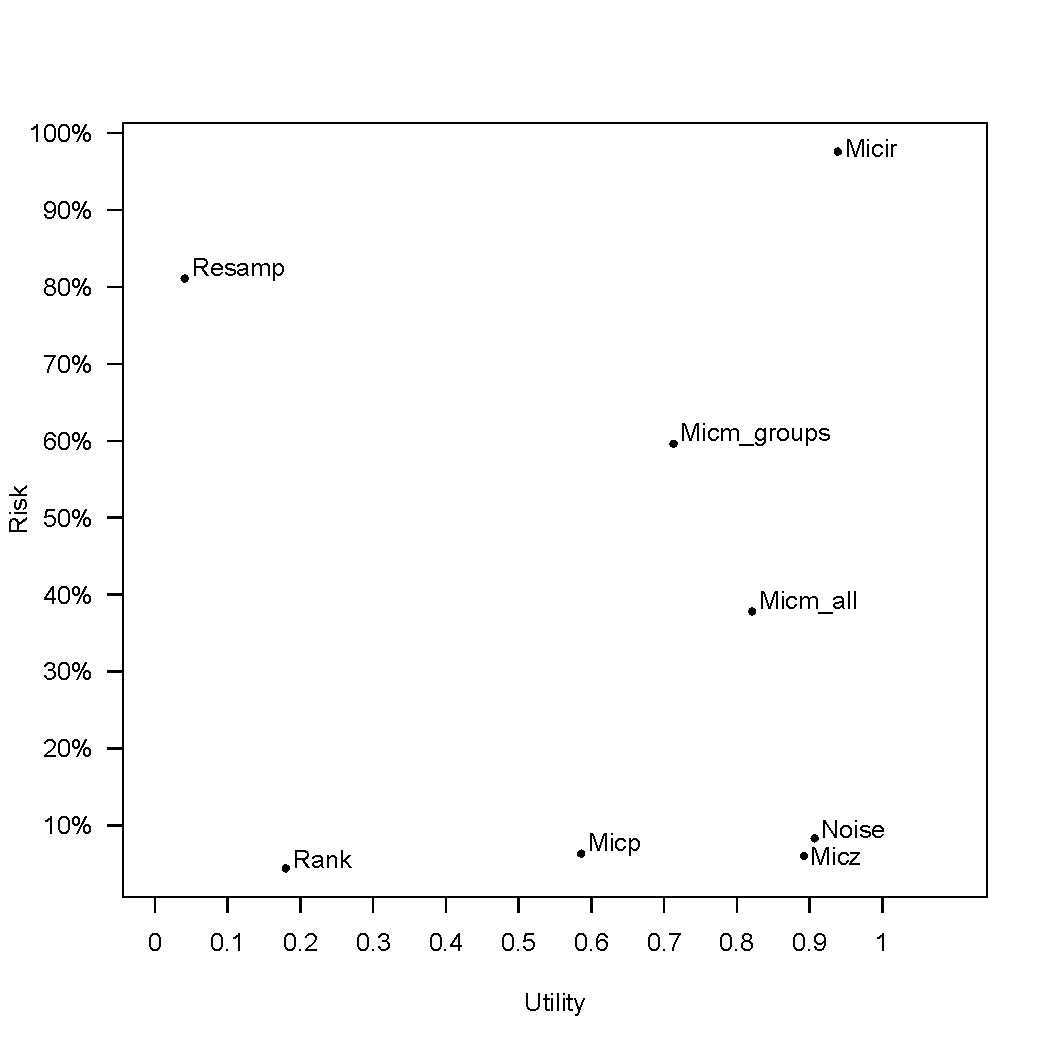
\includegraphics[width=4in]{R_U_plot.pdf}
\end{center}
\caption{Risk-Utility plot}
\label{fig.ruplot}
\end{figure}



\section{ Data Utility metrics} \label{du_metrics}
In this section we present some examples of Data Utility metrics \DU\ that can be used by the data protector to assess the quality of the masked data, which can help to choose an appropriate approach for disclosure limitation.

\subsection{Global metrics... This section is still under construction.... }


Global metrics capture global differences between the distributions of the original and masked
data. To access such global differences between the distributions of the original and masked 
data one could use for example Kullback-Leibler divergence.  
When the data are approximately multivariate normal, the \KL\
captures the differences in the distributions of the entire data,
which in turn account for differences in inferences. 
However, the \KL\ measure is not easily
interpreted when the data, or some transformed version of the
data, are not reasonably well-described by a multivariate normal
distribution, that is why it's  usage as  global metric of data utility
would be limited.

$ $
 
 {\bf Propensity score metric (which is an example of a generic metric)  will be added here...}

$ $

Generic metrics may be blunt in that they do not necessarily distinguish 
among variables. For example, an \SDL\ procedure that produces very different
distributions for a subset of substantively important predictors,
but matches well on the subset of substantively unimportant
predictors, could be rated as higher utility than a procedure that
produces the opposite effects.  Similarly, minimizing the \KL\
value may not lead to optimal \DBREL\ for certain conditional
distributions.  


\subsection{Analysis specific metrics}
In this section we describe several analysis-specific or so called ``narrow" measures of data utility. There are many possible ways of defining such type of metrics,  they 
are linked to the types of analyses the user would like to do on the original data.
 Obviously, we cannot cover all of them, so below we present some examples 
 that can help to illustrate the idea of such metrics.



\subsection{Confidence Interval Overlap Utility Measures}\label{subsec.ci}

Data users and analysts  are frequently interested in fitting regression models. 
This process produces not only point estimates of the coefficients, but
confidence intervals as well. Thus, it is desirable for utility measures 
to indicate when the inferences, and
not just the point estimates, from regressions using the released
data are close to the corresponding ones using the original data.

Confidence intervals are main mechanism of inference in regression
models. Therefore, one measure of utility is the degree of overlap
between confidence intervals obtained from the same regressions
fit using the \DBREL\ and \DBORIG. The greater the overlap, the
higher the utility.

\subsubsection{Interval Overlap Metric}
Consider a fixed regression on the data, with specified response
and predictors. Let $(L_{\mathrm{rel},k}, U_{\mathrm{rel},k})$ be
the lower and upper limits of the 95\% confidence interval for the
regression coefficient $\beta_{k}$ obtained from \DBREL, and let
$(L_{\mathrm{orig},k}, U_{\mathrm{orig},k})$ be the corresponding
interval obtained from \DBORIG. Let $f_{\mathrm{rel},k}$ and
$f_{\mathrm{orig},k}$ be the estimated posterior distributions of
$\beta_k$ computed under \DBREL\ and \DBORIG, respectively.  For
example, in linear regression, $f_{\mathrm{orig},k}$ is the usual
$t$-distribution on $n-p$ degrees of freedom with mean
$\hat{\beta}_{\mathrm{orig},k}$ and variance the $k$th diagonal
element in
$\hat{\sigma}^2_{\mathrm{orig}}\left(X^{'}_{\mathrm{orig}}
X_{\mathrm{orig}}\right)^{-1}$, where
$\hat{\sigma}^2_{\mathrm{orig}}$ is the estimated residual
variance obtained from fitting the regression of
$Y_{\mathrm{orig}}$ on the associated $n \times p$ matrix of
predictors, $X_{\mathrm{orig}}$, which includes a vector of ones
for the intercept.

The probability overlap in the confidence intervals for
any $\beta_{k}$ \citep{kkors06} is defined to be equal to:
\begin{equation}
I_k = \frac{1}{2}
\left[\int_{L_{\mathrm{rel},k}}^{U_{\mathrm{rel},k}}
f_{\mathrm{orig},k}(t) dt +
\int_{L_{\mathrm{orig},k}}^{U_{\mathrm{orig},k}}
f_{\mathrm{rel},k}(t) dt \right]
\end{equation}
and the interval overlap measure, \IO, as
\begin{equation}
I = \sum_{i=1}^p I_k / p
\end{equation}
where $p$ is the dimension of the predictor variable matrix, including
the intercept.

By design, $0 \leq I_k \leq 0.95$ (as is the case for $I$), with
effectively no overlap corresponding to $I_k =0$ and perfect
overlap corresponding to $I_k = 0.95$.  Averaging the two
integrals in the definition of $I_k$ helps deal with cases where
$(L_{\mathrm{orig},k}, U_{\mathrm{orig},k}) \subseteq
(L_{\mathrm{rel},k}, U_{\mathrm{rel},k})$, or vice versa.  For an
illustrative example, consider the case where
$(L_{\mathrm{orig},k}, U_{\mathrm{orig},k}) = (8, 10)$, and for
two different proposed releases the $(L_{\mathrm{rel_1},k},
U_{\mathrm{rel_1},k})=(-12, 30)$ and $(L_{\mathrm{rel_2},k},
U_{\mathrm{rel_2},k})=(3, 15)$. From a utility perspective, the
second release is clearly preferable over the first release. The
\IO\ as defined favors the second release.  A criterion that just
equals $\int_{L_{\mathrm{rel},k}}^{U_{\mathrm{rel},k}}
f_{\mathrm{orig},k}(t) dt$ does not clearly distinguish the
releases, since this integral for both procedures is essentially
one. Similar examples can be constructed to show the inadequacy of
using $\int_{L_{\mathrm{orig},k}}^{U_{\mathrm{orig},k}}
f_{\mathrm{rel},k}(t) dt$ alone.

The \IO\ does not distinguish among intervals that have $I_k$
essentially equal to zero, some of which may be ``less worse''
than others. To adjust for this, the measure can be modified by
adding some distance-based penalty when $I$ is essentially zero,
or perhaps even when $I_k$ is essentially zero for some $k$, where
distance is defined as some function of the
$|\hat{\beta}_{\mathrm{rel},k} - \hat{\beta}_{\mathrm{orig},k}|$
or of $\min\left\{|L_{\mathrm{rel},k} - U_{\mathrm{orig},k}|,
|L_{\mathrm{orig},k} - U_{\mathrm{rel},k}|\right\}$.

An alternative measure is the overlap in the interval lengths. Let
$(L_{\mathrm{over},k}, U_{\mathrm{over},k})$ be the overlap in
these intervals, defined as $\left\{b: b \geq L_{\mathrm{orig},k},
b \geq L_{\mathrm{rel},k},  b \leq U_{\mathrm{orig},k},  b \leq
U_{\mathrm{rel},k}\right\}$. Then, the average relative overlap in
the confidence intervals for any $\beta_{k}$ equals:
\begin{equation}
J_k = \frac{1}{2} \left[\frac{U_{\mathrm{over},k} -
L_{\mathrm{over},k}}{U_{\mathrm{orig},k} - L_{\mathrm{orig},k}} +
\frac{U_{\mathrm{over},k} -
L_{\mathrm{over},k}}{U_{\mathrm{rel},k} -
L_{\mathrm{rel},k}}\right].
\end{equation}
The interval overlap measure then could be defined as $J = (1/p)
\sum_{i=1}^p J_k$.

\subsubsection{Ellipsoid Overlap Metric}\label{subsec.overlap}
The \IO\ measure considers each interval separately, effectively using all
the conditional distributions of the coefficients rather than
their joint distribution. Some analysts may be interested in
simultaneous intervals, which are defined by multidimensional
ellipsoids.  So, ellipsoid overlap measure \EO\ is constructed 
based on  posterior probabilities of regions defined by ellipsoids, that is, 
Bayesian perspective is used.  Generically, let $\hat{\beta}$ be the
maximum likelihood estimate of $\beta$, the $p \times 1$ vector of
true coefficients in the regression of $Y$ on $X$, and let
$\hat{\sigma}^2$ be the estimated residual variance for that
regression. Under the standard linear regression assumptions and
assuming standard non-informative prior distributions for $\beta$
and $\sigma^2$, the $(1-\alpha)100\%$ joint highest posterior
density ellipsoid for $\beta$ is defined by all the values of
$\beta$ such that
\begin{displaymath}\label{eq_1}
\frac{(\beta
-\hat{\beta})^T(X^{T}X)(\beta-\hat{\beta})}{p\hat{\sigma}^2} \leq
F(\alpha;p, n-p)
\end{displaymath}
where $F(\alpha;p, n-p)$ is the critical value from the $F$
distribution with $p$ and $n-p$ degrees of freedom.  The ellipsoid
from the \DBORIG, which we call $E_{\mathrm{orig}}$, is obtained
by setting $\hat{\beta} = \hat{\beta}_{\mathrm{orig}}$,
$\hat{\sigma}^2 = \hat{\sigma}^2_{\mathrm{orig}}$, and $X =
X_{\mathrm{orig}}$. The ellipsoid from the \DBREL, which we call
$E_{\mathrm{rel}}$, is obtained by setting $\hat{\beta} =
\hat{\beta}_{\mathrm{rel}}$, $\hat{\sigma}^2 =
\hat{\sigma}^2_{\mathrm{rel}}$, and $X = X_{\mathrm{rel}}$.

The utility measure \EO\ is the average of two posterior
probabilities: 1) the probability of $E_{\mathrm{orig}}$ computed
using the posterior distribution of $\beta$ based on \DBREL, and
2) the probability of $E_{\mathrm{rel}}$ computed using the
posterior distribution of $\beta$ based on \DBORIG. To determine
these probabilities,  Monte Carlo simulations can be used. For the first
probability, we draw values of $\beta$ from its posterior
conditional on \DBREL\ which is a $p$-variate t-distribution with
mean $\hat{\beta}_{\mathrm{rel}}$ and covariance matrix
$\hat{\Sigma}_{\mathrm{rel}} =
\hat{\sigma}^2_{\mathrm{rel}}(X_{\mathrm{rel}}^{t}X_{\mathrm{rel}})^{-1}$
with $n-p$ degrees of freedom. We then calculate the percentage of
these drawn $\beta$ that lie within $E_{\mathrm{orig}}$.  A
similar process is used to obtain the second probability by
drawing from the posterior of $\beta$ given \DBORIG\ and finding
the percentage of these that lie inside $E_{\mathrm{rel}}$. As
with \IO, the \EO\ can be extended to any parameters whose
distribution is well-approximated by a multivariate normal
distribution.

% Here: start removing from here or drastically reducing, we may just say that 
% such and such methods have generally such and such utility or compare in such a way with other methods,
% say noise is better than mixroaggregation and microaggregation is better than swapping - or simething like that.

\subsection{On Utility Properties of some families of \SDL\ methods}
\label{subsec.simulateddata}

There is a wide plethora of SDL methods and they differ significantly in terms of utility  and risk. Another source of variability of SDL methods in terms of utility (and risk as well) is due to the fact that SDL methods can be applied with a different degree of intensity, that is, data protector can chose  different values of parameters for these methods. 
For example, for Noise addition, smaller or larger variance of Noise can be chosen, which will affect the utility and risk of the masked data. For Swapping, the percentage of swapped records can be different, for Rankswappping  the  maximal allowed difference in the ranks of the swapped records  may vary (which is a parameter of Rankswapping). For Microaggregation, a minimal number of records per group should be set up by the data protector.  There is a wide variety of SDL methods and  infinitely many method-parameter combinations each leading to a masked data set with different utility and risk. Hence, we do not intend to provide a comprehensive utility comparisons here, but instead to present some examples of generic utility characterizations of different families of SDL methods . 

One of the largest families of SDL methods (in terms of different  implementations) is a  Microaggregation family. It can   be divided into Multivariate Microaggregation   and  Univariate Microaggregation. The later group includes Microaggregation with individual ranking which consists of microaggregating each variable individually and independently from other variables and Microaggregation using projections. The later one is usually accomplished by ranking  multivariate data by projecting them onto a single axis, using either the sum of $z$-scores or the first principal component, and then aggregating data into groups of size $k$, except possibly for one group of larger size (from $k+1$ to $2k -1$).
Of all these methods, Microaggregation with individual ranking is typically the least perturbative method \citep{kkors06}. Typically, masked values obtained using this method are close to the corresponding original ones, and thus analyses performed on the masked data often lead to a very similar results to those obtained on the original data. For example, \EO\ utility metric is often high (close to $1$)  for this method \citep{kkors06}. On the other hand, the risk of re-identification using record linkage approach is high for this method as well. 
In contrast to Microaggregation using Individual Ranking, projection-based Microaggregation methods and Multivariate Microaggregation may introduce significant perturbation to the data with utility ranging from average to low according to \IO\ and \EO\ . But the re-identification risk (estimated based on record-linkage experiments) is low as well \citep{}. 

One of the desirable features of Microaggregation methods is that they  inherently satisfy requirements of k-anonymity (if this criterion for Risk  is adopted by the data protector of course). Also microaggregation methods preserve means of the original data, they preserve positivity/non-negativity  constraints in the data (if the original values are positive, so are the masked values)  which in some instances of data release  is a desirable feature. Microaggregation methods, on the other hand have a shrinking effect on the original data by reducing  the variance of the original data.
 
 $ $ 

{\bf To be continued... A few more SDL families will be described/compared in terms of Utility}
 
 \bibliographystyle{apalike}
\bibliography{dg2-new}

%%%%%%%%%%
 %%
\def\thisfile{times_tpl-new.tex}
\def\thisfiledate{2020/03/18}
\typeout{***** `\thisfile' <\thisfiledate> *****}
\end{document}
